\chapter{Algorithm }
\section{Functionality}
The algorithm consists of three phases. In the first phase, an entire image is scanned to find prominent pixels, whose coordinates are stored in a vector. In the following images, the algorithm just calculates these specific points and checks if this point is still considered to be prominent. If there are too many points which are not prominent anymoore, a change is triggered phase 3 starts which waits until the number of edges stabilizes. 

\subsection{Phase 1; Finding pixels of interest}
To find the pixels of interest (POI), the entire image is scanned with parts of the Harris edge filter.  But instead of finding local maximums to detect the corners, the algorithm divides the image into a configurable amount of subsections, horizontally and vertically. Each subsection is scanned for it's biggest corner-value. If this value exceeds a predefined threshold, his coordinates and his value are stoored into a vector. This selection leads to a better distribution accross the image. 

\begin{figure}[h!]
	\centering
	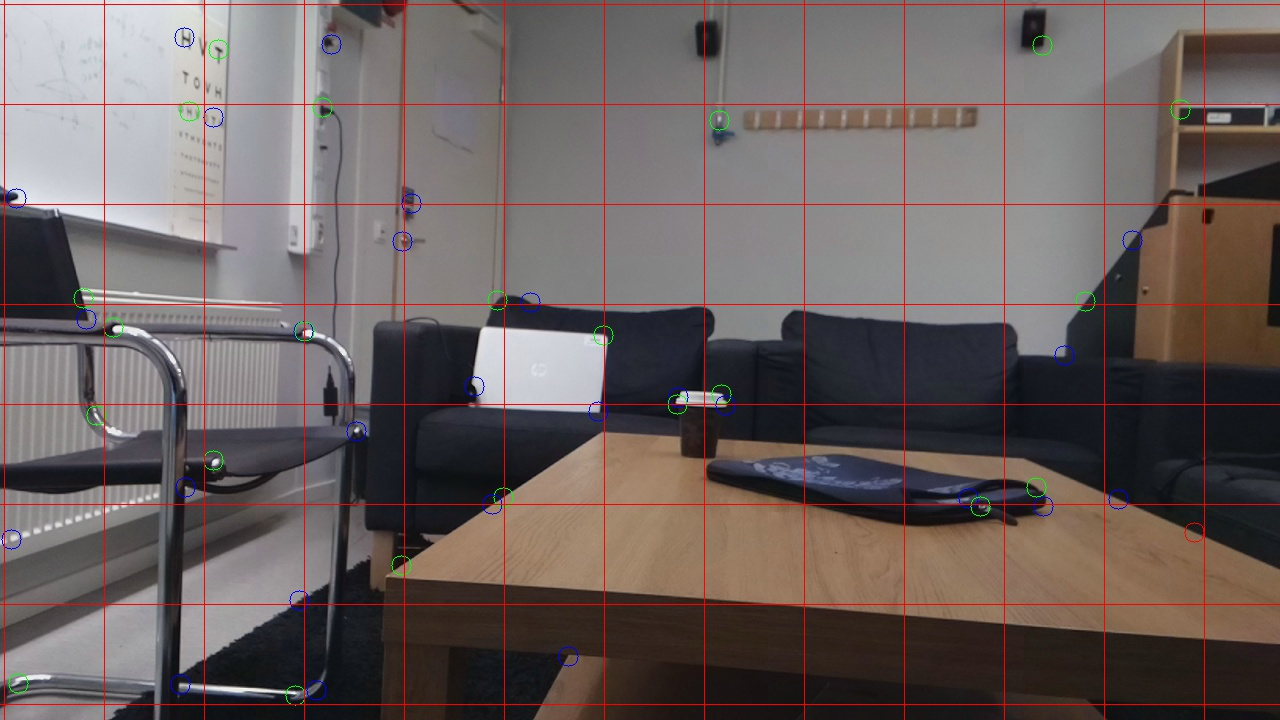
\includegraphics[width=0.9\linewidth]{bin/hotspots}
	\caption{Camera image with a overlay of found edges in each subsection. The red circle in the right bottom represents a point which isn't considered to be an edge anymore. }
	\label{fig:hotspots}
\end{figure} 


\subsection{Phase 2; Check pixels of interest}
From this point, just the coordinates stored in the vector which was created in phase 1 are calculated.  For each touple in the vector (e.g. x,y,value) newValue is determined in the new image at position x:y. When newValue is big enough relativ to the original value, the point which the touple represents is still considered to be an corner. This relative solution results in less noise then when comparing it again to the threshold used in Phase 1, because values close to the threshold were toggling to be a corner or not in some frames. Furthermoore, neighbour pixels of very strong edges were still considered to be edges, even though the image moved slightly. 

If the amount of missing corners becomes bigger than a percentage of the vectorsize, a changeStart is triggered and Phase 3 is entered.

\subsection{Phase 3;  Stabilize}
In the last phase, the algorithm waits untill the number of found edges stops changing for 3 Frames in a row ($\pm$ 1 corner tolerance). During this phase the vector might be recalculated as well if there are not enough matches.

\subsection{Why Harris}
Compared to simple Edge-Filters as Sobel or Prewitt, Harris finds corners where edges from Prewitt- or Sobelfilters are coming together. Therefore they are fragile to changes in all directions, whereas sobel and Prewitt are not fragil when the camera moves along the edges. The chance of accidentally hitting another Harris corner is very small.



\section{Influences}
\subsection{Light changes}
Because the algorithm operates on the corner-values, it is not vulnerable to small light changes. If light changes often causes unwanted change events, the algorithm might be extended to operate on the color images of YUV instead of the grayscale image. But this was not covered within this project.

\subsection{Slow movement}
By selecting fixed points, this solution can also detect very slow changes of the camera, which is a requirement of a changesystem who should trigger a recalibration.

\subsection{ Partial changes}
As stated out in the requirements, the algorithm shouldn't trigger a change if just parts of the scene are moving or overlapped. 
\subsubsection{Distribution}
To achieve this tolerance it is important, that the POIs are well distributed over the image, which is assured by dividing the image into a grid to find maximums instead of finding local maximums, as suggested in the original Harris-Filter. Otherwise, a small object might overlap multiple important points which results in a change event.
\subsubsection{ Emphasis }
Furthermoore it is important that all POIs have the same significance. Instead of comparing the sum up of all POI-Value-Differences compared with the Phase1 image, we count the amount of Points which are still considered to be edges in the new image.


\chapter{Technical decisions}
\section{Halide}
Because the same algorithm must run over the entire image in the first place and afterwards over specific pixels only, it is important that the  algorithm could handle both tasks in order to avoid the effort of programming everything twice and, more imprtant, assure that it always has the same result. 

\subsection{32 Bit Kernel}
Even though the Raspberry PI 3 has a 64bit processor, at the time of writing, there are no mature linux distributions with a 64bit kernel out there for the raspberry. As soon as they're available, I would suggest to switch to a 64Bit kernel in order to take advantage of many additional CPU-registers for better performance.

\section{Type casting}
As shown bellow, C doesn't handle overflows consistently. Even thought it is a 64 Bit System, which was determined by printing sizeof($int^*$), overflows in uint8\_t were preserved on shift back whereas uint32\_t looses this information. Even thought this project might benefit from using 8bit calculations, 8 bit values are casted to 16 bit before a calculation whose intermediate results exceed 255 to assure a portable and stable solution.

\begin{minted}[linenos=true]{cpp}
#include <stdio.h>
#include <stdint.h>
#include <limits.h>

int main()
{
	uint32_t a = UULONG_MAX>>32,
		b = UULONG_MAX>>32,
		res = (uint32_t)((a+b)>>1);
	printf("Result(%lu): %lu\n", a, res);
	
	return 0;
}
\end{minted}
\textit{ Result (4294967295): 2147483647 \\
	(2\textsuperscript{32})-1: 2\textsuperscript{31}
}
\begin{minted}[linenos=true]{cpp}
#include <stdio.h>
#include <stdint.h>
#include <limits.h>

int main()
{
	uint8_t a = 255,
		b = 255,
	res = (uint8_t)((a+b)>>1);
	printf("Result(%u): %u\n", a,res);
	
	return 0;
}

\end{minted}
\textit{ Result(255): 255 } \\
To assure repeatability, this experiment was executed on \\ https://www.tutorialspoint.com/compile\_c\_online.php.


\chapter {Technical implementation}
\section{ Docker }
This project uses docker, a lightwight container virtualization solution, to develop and test the quality of the algorithms. All images used in this project are published on hub.docker.com. Because they are autobuilt, which means that hub.docker.com builds them out of so called Dockerfiles, you can reliably see, how these images are set up. In order to execute the provided commands, it is sufficient to have docker up and running. All required files will be downloaded if it is not available locally.

\section{Build process}
All required files are available under \enquote{https://github.com/mineichen/cameraChangeDetection}. The build process is split into two phases and is not fully automated yet.
 
\begin{enumerate}
	\item{ Generate the harris-filter as a static C library}
	\item{ Compile the GStreamer plugin which contains all the logic}
\end{enumerate}

In order to execute the build commands, the current working directory has to be the same as the project root directory.

\subsection{Harris-Filter}
The Harris-filter is build with the halide programming language. Because halide comes with a cross-compiler built in, the harris binaries for the development-platform and the raspberry pi are compiled inside of a halide-docker-container. The resulting static library inside build/*platform* doesn't have any dependencies to halide. To change the target platform, the \enquote{platform}-variable in halide/build.sh has to be changed.

\begin{lstlisting}[language=bash]
$ docker-compose run halide sh code/build.sh
\end{lstlisting}

For development purpose, the precompiler-condition in the main function could be changed to apply the algorithm to a single png image. 

\subsection{Gstreamer-Plugin}
Unlike the Harris filter, the Gstreamer-Plugin isn't prepared to be cross compiled. Therefore, the compilation is done on the platform by executing the \enquote{gstreamer/build.sh} script. For development purpose, the following command builds the dynamic-library, which has to be linked to gst-launch at runtime.

\begin{lstlisting}[language=bash]
docker-compose run gstreamer sh code/build.sh
\end{lstlisting}

The static Harris-Filter-library has to be copied into the gstreamer/lib/ folder to be found by the compiler. \enquote{gstreamer/codes.txt} contains useful gst-launch pipelines with examples.

\chapter{Results}
In this chapter, the amount of corners found in the scenes are documented. The red line in the diagrams represents the amount of corners expected to be found and the blue line represents the amount of corners actually found at the given coordinates. During the analysis, the parameter which determines, which percentage of the original edgevalue a following point has to have, to be considered a corner, had a big influence in the result. Therefore the following sections contain the result with the parameters 50\% on top and 75\% bellow. The red areas in the 75\% diagrams show the timespan between changeStart and changeEnd.

\section{Method}
The data used in the following diagrams is generated within a pipeline inside the gstreamer-plugin. In order to produce analytic data, the MIUN\_ANALYTIC precompiler variable has to be set to a non-zero value. Afterwards it produces the following files inside the \enquote{/gstreamer} folder:
\begin{description}
	\item[matches.data] 
	Each row represents one image in the test sequence. The columns contain the following values:
	\begin{enumerate}
			\item{Frameindex}
			\item{Number of corners found}
			\item{Number of corners expected}
			\item{Difference between courners found and expected}
	\end{enumerate}
	\item[poi.data] 
		Contains the coordinates of all POIs for each image and weather they are still considered to be corners on that particular image.
			\begin{enumerate}
			\item{Position X}
			\item{Position Y}
			\item{1 if still a corner, 0 if not a corner anymore}
		\end{enumerate}
		 
	\item[changes.data] 
		Each row in that file represents a change which consists of a startframeindex and a endframeindex. This data is used to benchmark the algorithm.
\end{description}

For visual feedback, the following command transforms the raw video data into enumerated jpg-images.

\begin{lstlisting}[language=bash]
docker-compose run gstreamer gst-launch-1.0 \
  filesrc location=data/raw/camVertMove.yuv \
  ! videoparse width=1280 height=720 format=2 \
  ! jpegenc \
  ! multifilesink location=data/sequence/verticalMove/im%06d.jpg
\end{lstlisting}

\section{Scenes}
\subsection{Bump}
The algorithm works very precisely in that situation. It hasn't missed a single bump or triggered one when there was any. All project goals are achieved.

\begin{tikzpicture}
	\begin{axis}[
          width=\linewidth, % Scale the plot to \linewidth
          height=200,
          grid=major, % Display a grid
          grid style={dashed,gray!30}, % Set the style
          xlabel=Framenumber, % Set the labels
          ylabel=Nr. of matching points,
          %x unit=\si{\volt}, % Set the respective units
          %y unit=\si{\ampere},
          legend style={at={(0.5,-0.2)},anchor=north}, % Put the legend below the plot
          x tick label style={anchor=north,yshift=-2}, % Display labels sideways
          y tick label style={anchor=east,xshift=-2},
          ymin=0,
          xmin=0,
          xmax=200
        ]
		\addplot table [x=frame,y=points, col sep=comma	] {data/bump/final.csv};
		\addplot table [x=frame, y=total, col sep=comma] {data/bump/final.csv};
	\end{axis}
\end{tikzpicture}

\begin{tikzpicture}
\begin{axis}[
width=\linewidth, % Scale the plot to \linewidth
height=200,
grid=major, % Display a grid
grid style={dashed,gray!30}, % Set the style
xlabel=Framenumber, % Set the labels
ylabel=Nr. of matching points,
%x unit=\si{\volt}, % Set the respective units
%y unit=\si{\ampere},
legend style={at={(0.5,-0.2)},anchor=north}, % Put the legend below the plot
x tick label style={anchor=north,yshift=-2}, % Display labels sideways
y tick label style={anchor=east,xshift=-2},
ymin=0,
xmin=0,
xmax=200
]
\addplot+[
	emphasize=8:11 with red!10,
	emphasize=24:35 with red!10,
	emphasize=41:45 with red!10,
	emphasize=59:65 with red!10,
	emphasize=78:83 with red!10,
	emphasize=93:99 with red!10,
	emphasize=107:116 with red!10,
	emphasize=121:127 with red!10,
	emphasize=135:140 with red!10,
	emphasize=148:155 with red!10,
	emphasize=161:167 with red!10,
	emphasize=175:181 with red!10,
	emphasize=188:193 with red!10,
	emphasize=202:212 with red!10,
] table [x=frame, y=points, col sep=comma] {data/bump/final3div4.csv};
\addplot table [x=frame, y=total, col sep=comma] {data/bump/final3div4.csv};
\end{axis}
\end{tikzpicture}

\subsection{Scene change}
In that sequence, there was no change triggered. The lowest amount of matching points was reached in Frame 630, where someone moved the chair which held many POIs in the scene. The black notebook-bag was moved permanently in frame number 470. 

This shows, that the algorithm has a weakness for permanent changes in the scene. If too many of these happen, a change will trigger faster. 

Even tought a change was almost triggered in frame 630, there was no false positive and no false negative.


\begin{figure}[h!]
	\centering
	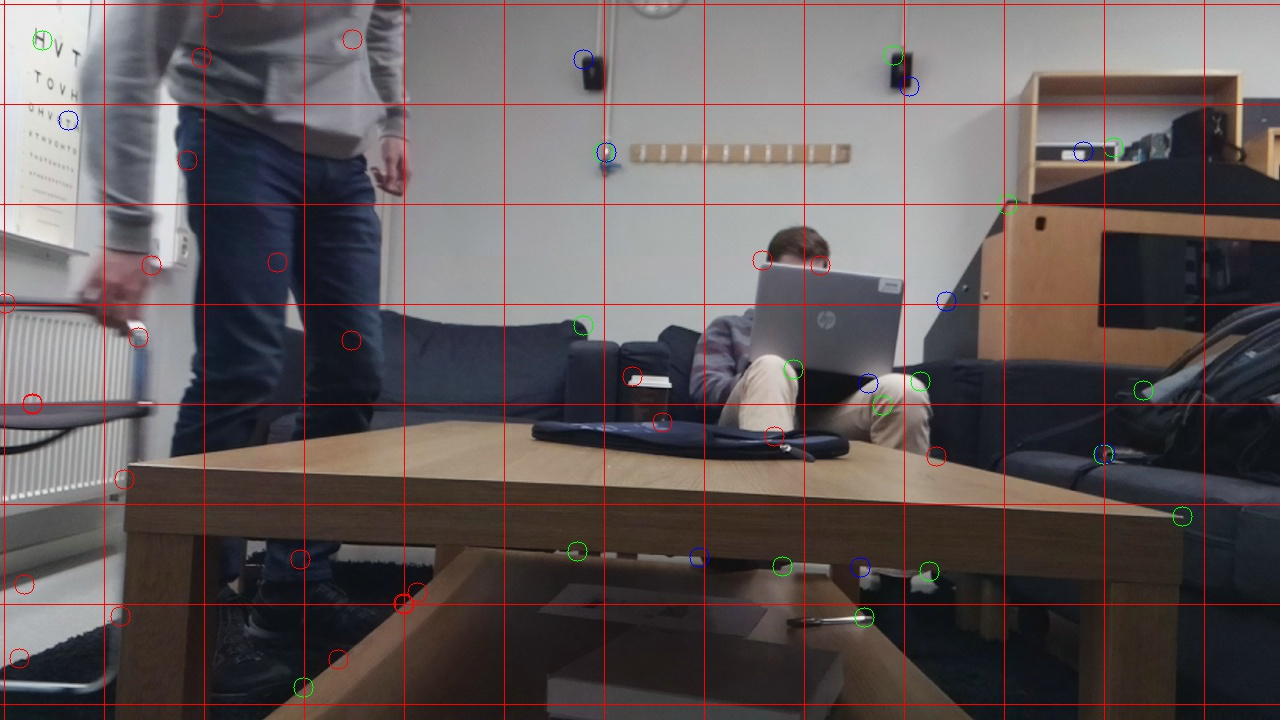
\includegraphics[width=0.9\linewidth]{bin/changeSceneWorst}
	\caption{Worst performance in changeScene sequence. Red Circle means not found anymore. Green and blue is used in a chess-like pattern to distinguish to which subsection a circle belongs to.}
	\label{fig:hotspots}
\end{figure} 


\begin{tikzpicture}
	\begin{axis}[
          width=\linewidth, % Scale the plot to \linewidth
          height=200,
          grid=major, % Display a grid
          grid style={dashed,gray!30}, % Set the style
          xlabel=Framenumber, % Set the labels
          ylabel=Nr. of matching points,
          %x unit=\si{\volt}, % Set the respective units
          %y unit=\si{\ampere},
          legend style={at={(0.5,-0.2)},anchor=north}, % Put the legend below the plot
          x tick label style={anchor=north,yshift=-2}, % Display labels sideways
          y tick label style={anchor=east,xshift=-2},
          ymin=0,
          xmin=0,
          xmax=1500
        ]
		\addplot table [x=frame, y=points, col sep=comma] {data/sceneChange/final.csv};
		\addplot table [x=frame, y=total, col sep=comma] {data/sceneChange/final.csv};
	\end{axis}
\end{tikzpicture}


\begin{tikzpicture}
\begin{axis}[
width=\linewidth, % Scale the plot to \linewidth
height=200,
grid=major, % Display a grid
grid style={dashed,gray!30}, % Set the style
xlabel=Framenumber, % Set the labels
ylabel=Nr. of matching points,
%x unit=\si{\volt}, % Set the respective units
%y unit=\si{\ampere},
legend style={at={(0.5,-0.2)},anchor=north}, % Put the legend below the plot
x tick label style={anchor=north,yshift=-2}, % Display labels sideways
y tick label style={anchor=east,xshift=-2},
ymin=0,
xmin=0,
xmax=1500
]
\addplot table [x=frame, y=points, col sep=comma] {data/sceneChange/final3div4.csv};
\addplot table [x=frame, y=total, col sep=comma] {data/sceneChange/final3div4.csv};
\end{axis}
\end{tikzpicture}

\pagebreak 

\subsection{NoChange}
The following diagrams show that the algorithm doesn't trigger any unnecessary changes if the scene is not changed and the camera not touched.

\begin{tikzpicture}
	\begin{axis}[
          width=\linewidth, % Scale the plot to \linewidth
          height=200,
          grid=major, % Display a grid
          grid style={dashed,gray!30}, % Set the style
          xlabel=Framenumber, % Set the labels
          ylabel=Nr. of matching points,
          %x unit=\si{\volt}, % Set the respective units
          %y unit=\si{\ampere},
          legend style={at={(0.5,-0.2)},anchor=north}, % Put the legend below the plot
          x tick label style={anchor=north,yshift=-2}, % Display labels sideways
          y tick label style={anchor=east,xshift=-2},
          ymin=0,
          xmin=0,
          xmax=1500
        ]
		\addplot table [x=frame, y=points, col sep=comma] {data/noChange/final.csv};
		\addplot table [x=frame, y=total, col sep=comma] {data/noChange/final.csv};
	\end{axis}
\end{tikzpicture}

\begin{tikzpicture}
\begin{axis}[
width=\linewidth, % Scale the plot to \linewidth
height=200,
grid=major, % Display a grid
grid style={dashed,gray!30}, % Set the style
xlabel=Framenumber, % Set the labels
ylabel=Nr. of matching points,
%x unit=\si{\volt}, % Set the respective units
%y unit=\si{\ampere},
legend style={at={(0.5,-0.2)},anchor=north}, % Put the legend below the plot
x tick label style={anchor=north,yshift=-2}, % Display labels sideways
y tick label style={anchor=east,xshift=-2},
ymin=0,
xmin=0,
xmax=1500
]
\addplot table [x=frame, y=points, col sep=comma] {data/noChange/final3div4.csv};
\addplot table [x=frame, y=total, col sep=comma] {data/noChange/final3div4.csv};
\end{axis}
\end{tikzpicture}

\pagebreak 
\subsection{Horizontal Move}
Because of the recording technique, this sequece contains not only horizontal, but also many rotation movements. Somethimes there is no time to stabilize which leads to very long timeintervals between startChange and endChange events.

12 times the pause between the movements was too short and/or bumpy so that two movements were considered to be one long movement. There was no change which happened not in between a startChange and endChange event. 

At index 508 the algorithm triggered a movement which wasn't one. But 1/1547 is still under the threshold of 1\% and the project goals are therefore fulfilled in this sequence as well.

\begin{tikzpicture}
\begin{axis}[
width=\linewidth, % Scale the plot to \linewidth
height=200,
grid=major, % Display a grid
grid style={dashed,gray!30}, % Set the style
xlabel=Framenumber, % Set the labels
ylabel=Nr. of matching points,
%x unit=\si{\volt}, % Set the respective units
%y unit=\si{\ampere},
legend style={at={(0.5,-0.2)},anchor=north}, % Put the legend below the plot
x tick label style={anchor=north,yshift=-2}, % Display labels sideways
y tick label style={anchor=east,xshift=-2},
ymin=0,
xmin=0,
xmax=100
]
\addplot table [x=frame, y=points, col sep=comma] {data/horizontalMove/final.csv};
\addplot table [x=frame, y=total, col sep=comma] {data/horizontalMove/final.csv};
\end{axis}
\end{tikzpicture}

	
\begin{tikzpicture}
\begin{axis}[
width=\linewidth, % Scale the plot to \linewidth
height=200,
grid=major, % Display a grid
grid style={dashed,gray!30}, % Set the style
xlabel=Framenumber, % Set the labels
ylabel=Nr. of matching points,
%x unit=\si{\volt}, % Set the respective units
%y unit=\si{\ampere},
legend style={at={(0.5,-0.2)},anchor=north}, % Put the legend below the plot
x tick label style={anchor=north,yshift=-2}, % Display labels sideways
y tick label style={anchor=east,xshift=-2},
ymin=0,
xmin=0,
xmax=100
]
\addplot+[
	emphasize=1:8 with red!10,
	emphasize=14:20 with red!10,
	emphasize=32:57 with red!10,
	emphasize=62:72 with red!10,
	emphasize=78:92 with red!10
] table [x=frame, y=points, col sep=comma] {data/horizontalMove/final3div4.csv};
\addplot table [x=frame, y=total, col sep=comma] {data/horizontalMove/final3div4.csv};
\end{axis}
\end{tikzpicture}


\pagebreak 
\subsection{Vertical Move}
In this sequence it happens as well that two changes are summarized to one big movement ($~$18 Times). Specially at the end of the sequence, when the pause between the movements becomes smaller. But there was no bad detection and none happened not in between changeStart and changeEnd. There was no false Positive in this section. All the project goals are fulfilled.

\begin{tikzpicture}
\begin{axis}[
width=\linewidth, % Scale the plot to \linewidth
height=200,
grid=major, % Display a grid
grid style={dashed,gray!30}, % Set the style
xlabel=Framenumber, % Set the labels
ylabel=Nr. of matching points,
%x unit=\si{\volt}, % Set the respective units
%y unit=\si{\ampere},
legend style={at={(0.5,-0.2)},anchor=north}, % Put the legend below the plot
x tick label style={anchor=north,yshift=-2}, % Display labels sideways
y tick label style={anchor=east,xshift=-2},
ymin=0,
xmin=0,
xmax=100
]
\addplot table [x=frame, y=points, col sep=comma] {data/verticalMove/final.csv};
\addplot table [x=frame, y=total, col sep=comma] {data/verticalMove/final.csv};
\end{axis}
\end{tikzpicture}
\begin{tikzpicture}
\begin{axis}[
width=\linewidth, % Scale the plot to \linewidth
height=200,
grid=major, % Display a grid
grid style={dashed,gray!30}, % Set the style
xlabel=Framenumber, % Set the labels
ylabel=Nr. of matching points,
%x unit=\si{\volt}, % Set the respective units
%y unit=\si{\ampere},
legend style={at={(0.5,-0.2)},anchor=north}, % Put the legend below the plot
x tick label style={anchor=north,yshift=-2}, % Display labels sideways
y tick label style={anchor=east,xshift=-2},
ymin=0,
xmin=0,
xmax=100
]
\addplot+[
emphasize=5:14 with red!10,
emphasize=23:30 with red!10,
emphasize=39:48 with red!10,
emphasize=56:69 with red!10,
emphasize=74:83 with red!10,
emphasize=91:99 with red!10
] table [x=frame, y=points, col sep=comma] {data/verticalMove/final3div4.csv};
\addplot table [x=frame, y=total, col sep=comma] {data/verticalMove/final3div4.csv};
\end{axis}
\end{tikzpicture}


\section{Conclusion}
The algorithm works very reliably on the tested sequences, because all the project goals were achieved. Gstreamer allows a easy porting onto the raspberry pi. The biggest weakness of the algorithm are constant changes in the scene. If this causes problems in the future, recalculations of the whole image should be considered to happen in a specific interval. This can even occur subsection by subsection in order to distribute the system load. But it is important to consider, that very slow camera changes might not be detected anymore.

Because of the requirements to have a low false negative rate, the parameter 75\% should be favourized. However, both parameters had almost the same results in this sequences. 